\chapter{Exploratory Analysis}
In this chapter, I will copy the training  set to an exploratory set and 
work with it, because the exploratory analysis may require some data 
transformations, however I want to keep the training set untouched.

I will explore each attribute and its characteristics. Here is a list of
dataset attributes:
\begin{itemize}
	\item PassengerId
    \item Survived
    \item Pclass (page \pageref{section:Pclass})
    \item Name (page \pageref{section:Name})
    \item Sex (page \pageref{section:Sex})
    \item Age (page \pageref{section:Age})
    \item SibSp (page \pageref{section:SibSp})
    \item Parch (page \pageref{section:Parch})
    \item Ticket (page \pageref{section:Ticket})
    \item Fare (page \pageref{section:Fare})
    \item Cabin (page \pageref{section:Cabin})
    \item Embarked (page \pageref{section:Embarked})
\end{itemize}

I won't consider \textbf{"PassengerId"} and \textbf{"Survived"} attribures.
\textbf{"PassengerId"} attribute contains 891 passenger's IDs (see section 
\hyperref[section:first_rows]{First rows of the dataset} and table 
\ref{table:unique_values}), which won't help in building a model.
\textbf{"Survived"} attribute is a target. A passenger survived if their 
\textbf{"Survived"} attribute is 1, else the passenger drowned 
(\textbf{"Survived"} attribute is 0). Figure \ref{number_of_survivors}
shows numbers of survived and drowned passengers in whole dataset.


\section{Pclass} \label{section:Pclass}
The \textbf{Pclass} attribute contains information about socio-economic
status of the passenger:
\begin{itemize}
    \item 1st = Upper
    \item 2nd = Middle
    \item 3rd = Lower
\end{itemize}
Let's estimate the number of passengers of each class in the exploratory
set. The figure \ref{pic:pclass_count} illustrates this estimation.

\begin{figure}[!ht]
    \centering
    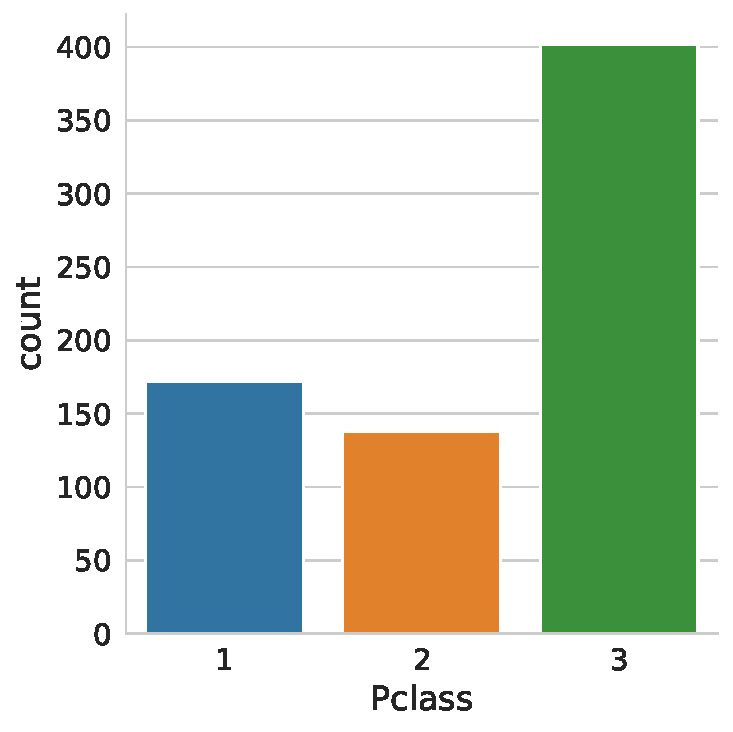
\includegraphics[width=0.5\textwidth]{pclass_count}
    \caption{Number of passengers in each \textbf{Pclass}}
    \label{pic:pclass_count}
\end{figure}

The figure \ref{pic:pclass_survived_entire_dataset} shows the proportions
of survived passengers for each \textbf{Pclass} in the exploratory set.

\begin{figure}[!ht]
    \centering
    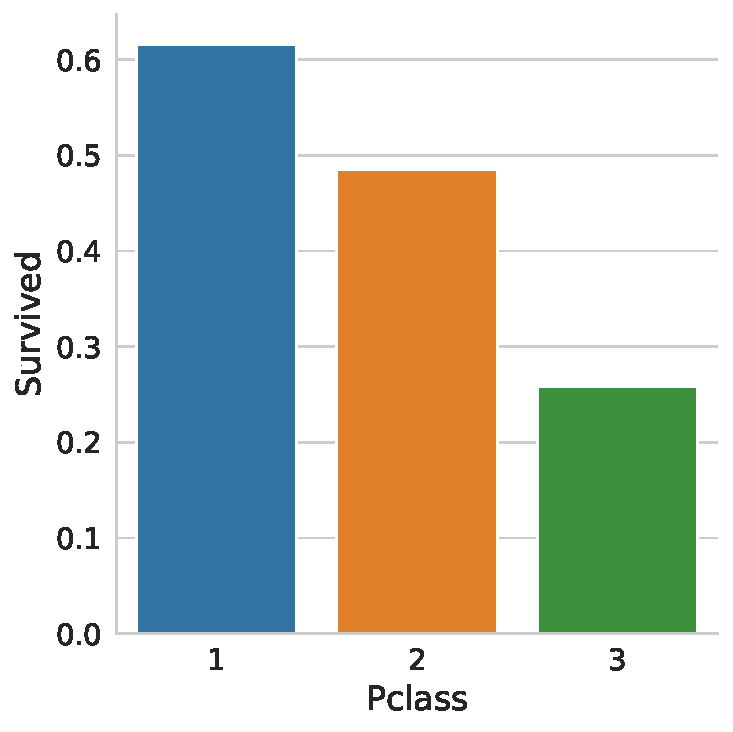
\includegraphics[width=0.5\textwidth]{pclass_survived_entire_dataset}
    \caption{Proportion of survived passengers in each \textbf{Pclass}}
    \label{pic:pclass_survived_entire_dataset}
\end{figure}

It looks like there were more passengers of the lower socio-economic class 
(\textbf{Pclass}=3), but they had less chance of surviving. \textbf{Pclass}
is a class of the ticket, so it contains information about the location 
of the passenger's cabin. It is known that the cabins of passengers with 
low socio-economic status were located on lower decks, that is, further 
from the lifeboats, this explains why there are fewer survivors among them
\cite{titanic-wikipedia}.

Finally, let's check the proportion of women among the survivors of each
\textbf{Pclass}. Figure \ref{pic:pclass_survived_gender} show these 
proportions.

\begin{figure}[!ht]
    \centering
    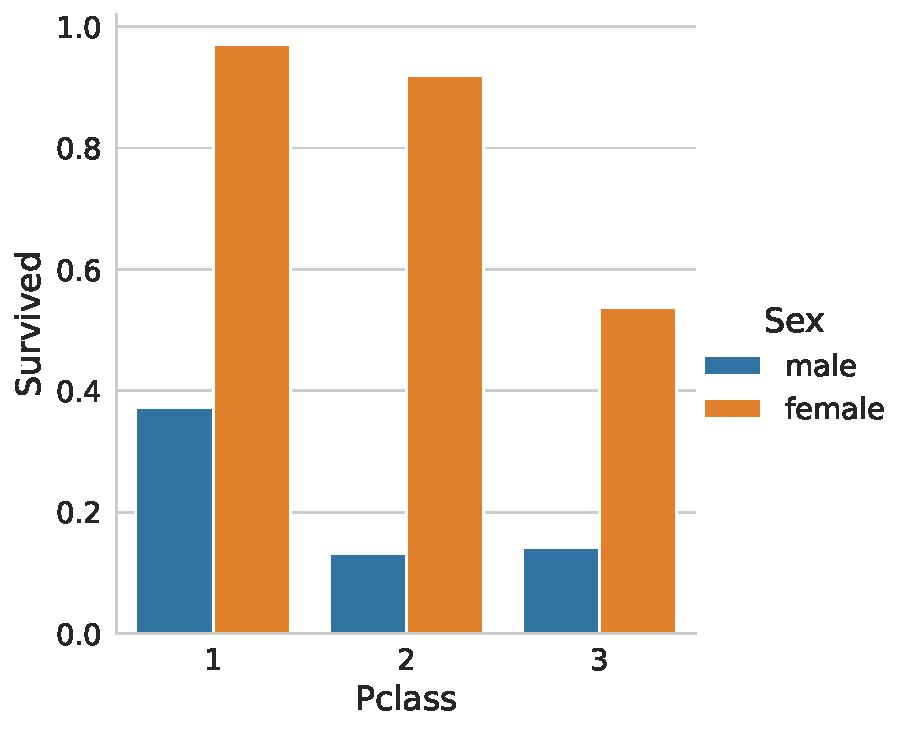
\includegraphics[width=0.5\textwidth]{pclass_survived_gender}
    \caption{Proportion of survived passengers of eache gender in each \textbf{Pclass}}
    \label{pic:pclass_survived_gender}
\end{figure}

More women than men survived in each \textbf{Pclass}.


\section{Name} \label{section:Name}

The \textbf{Name} attribute contains names of passengers, and it contains
712 unique values in the exploratory dataset. The table 
\ref{table:name_column_excerpt} shows the exerpt from this column. There 
seems to be a useful pattern. 

\begin{table}[!ht]
    \centering
    \caption{Excerpt from the \textbf{Name} column of the exploratory set}
    \begin{tabular}{|l|l|}
        \hline
                     & \textbf{Name}                             \\ \hline
        \textbf{788} & Dean, Master. Bertram Vere                \\ \hline
        \textbf{347} & Davison, Mrs. Thomas Henry (Mary E Finck) \\ \hline
        \textbf{629} & O'Connell, Mr. Patrick D                  \\ \hline
        \textbf{734} & Troupiansky, Mr. Moses Aaron              \\ \hline
        \textbf{106} & Salkjelsvik, Miss. Anna Kristine          \\ \hline
    \end{tabular}
    \label{table:name_column_excerpt}
\end{table}

Each name contains a title, such as "Mrs." or "Master.". The title may 
contain information about gender, socio-economic status, age, etc. Let's
extract the title from each name and count how many times each title occurs
in the exploratory set. The results is shown in the table 
\ref{table:titles_number} and figure \ref{pic:title_count}.

\begin{table}[!ht]
    \centering
    \caption{Number of occurrences of each title}
    \begin{tabular}{|
    >{\columncolor[HTML]{C0C0C0}}l |l|
    >{\columncolor[HTML]{C0C0C0}}l |l|}
    \hline
    \textbf{Title} & \textbf{Number} & \textbf{Title} & \textbf{Number} \\ \hline
    mr             & 415             & jonkheer       & 1               \\ \hline
    miss           & 144             & ms             & 1               \\ \hline
    mrs            & 88              & the countess   & 1               \\ \hline
    master         & 29              & don            & 1               \\ \hline
    dr             & 6               & mme            & 1               \\ \hline
    rev            & 4               & sir            & 1               \\ \hline
    major          & 2               & capt           & 1               \\ \hline
    col            & 2               & mlle           & 1               \\ \hline
    \end{tabular}
    \label{table:titles_number}
\end{table}

\begin{figure}[!ht]
    \centering
    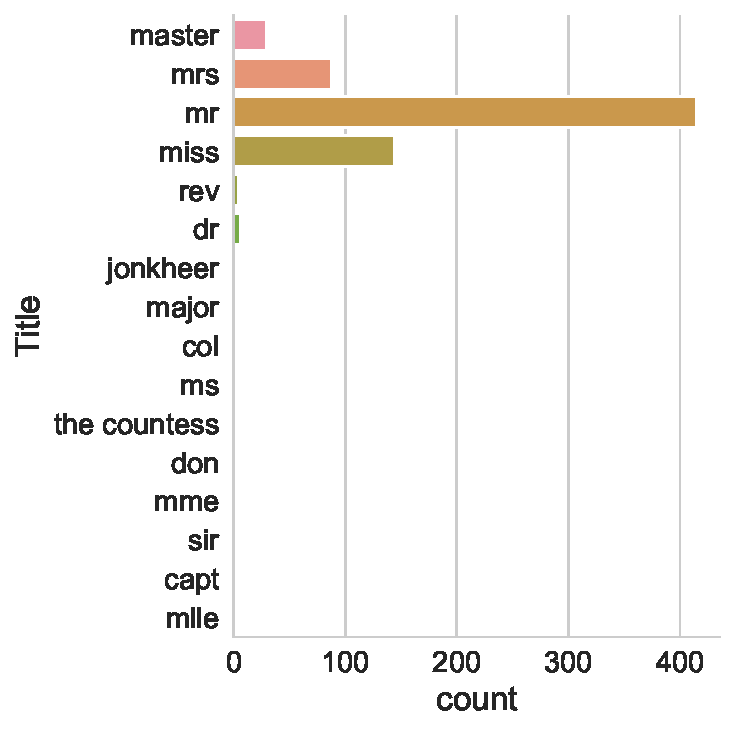
\includegraphics[width=0.5\textwidth]{title_count}
    \caption{Number of occurrences of each title}
    \label{pic:title_count}
\end{figure}

Several titles occurs extremely rarely, later we will combine them with 
more common titles.


\section{Sex} \label{section:Sex}
We have already studied this attribute in chapter \ref{chapter:sample_test_set}
"Sample a Test Set". Figures \ref{proportion_of_survived_women} and 
\ref{proportion_of_survived_women_among_pclasses} have shown that in the 
entire dataset and in each \textbf{"Pclass"} there are more female
survivors than males. So, it's very important attribute, and I will
consider other attributes separetely for each gender.


\section{Age} \label{section:Age}
Exploratory Analysis


\section{SibSp} \label{section:SibSp}
Exploratory Analysis


\section{Parch} \label{section:Parch}
Exploratory Analysis


\section{Ticket} \label{section:Ticket}
Exploratory Analysis


\section{Fare} \label{section:Fare}
Exploratory Analysis


\section{Cabin} \label{section:Cabin}
Exploratory Analysis


\section{Embarked} \label{section:Embarked}
Exploratory Analysis